\chapter{Budowa programu}
W rozdziale trzecim zawarto informacje dotyczące budowy programu. Na początku opisana jest jego struktura w postaci diagramów. Następnie opisane są poszczególne fragmenty programu. Na końcu znajduje się opis interfejsu graficznego programu.


\section{Struktura programu}

Poniżej znajduje się opis struktury plików oraz opis zawartości poszczególnych katalogów programu.

\begin{itemize}
	\item \textbf{photo-2-midi.py} - interfejs programu, uruchamia program.
	\item \textbf{convert\_to\_MIDI.py} - główna część programu, zarządza działaniem procesu uzyskiwania informacji ze zdjęć.
	\item \textbf{staff\_detection.py} - w skład tego pliku wchodzą funkcje odpowiedzialne za detekcję pięciolinii.
	\item \textbf{dewarp\_page.py} - plik zawierający całą logikę i działanie części programu odpowiedzialnej za usuwanie wypaczenia z obrazów wejściowych.
	\item \textbf{image\_segmentation.py} - jest plikiem posiadającym wszystkie funkcje mające za zadanie poprawne podzielenie obrazu na mniejsze fragmenty nadające się do przekazania dla wytrenowanego modelu uczenia maszynowego.
	\item \textbf{utils.py} - przechowuje funkcje dodatkowe.
	\item \textbf{trained\_model} - folder zawierający wytrenowany model uczenia maszynowego.
	\item \textbf{ML\_model/model} - folder przechowujące niezbędne pliki do użycia wytrenowanego modelu uczenia głębokiego.
\end{itemize}

\section{Diagram maszyny stanowej}
Poniżej przedstawiony jest diagram maszyny stanowej programu przy użyciu języka pół-formalnego UML.
\begin{figure}
	\centering
	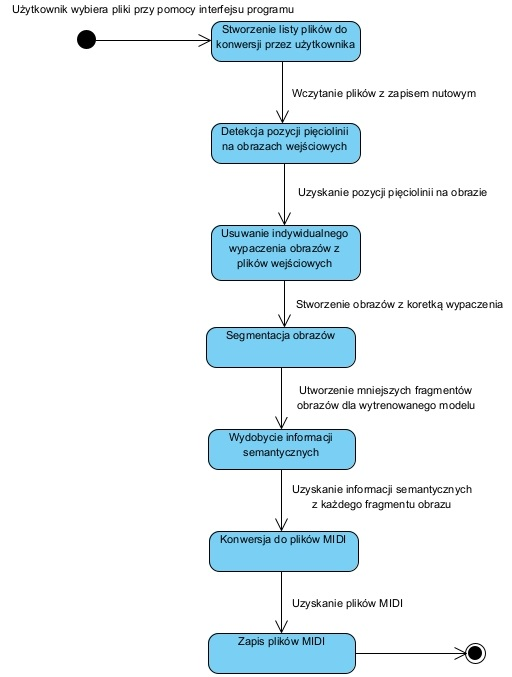
\includegraphics[width=10cm]{images/Diagram-maszyny-stanowej-programu.jpg}
	\caption{Diagram maszyny stanowej programu.}
	\label{fig:program-state-machine}
\end{figure}


\section{Przypadki użycia}
Poniżej przedstawiony jest diagram przypadków użycia programu przy użyciu języka pół-formalnego UML.

\begin{figure}[htb]
	\centering
	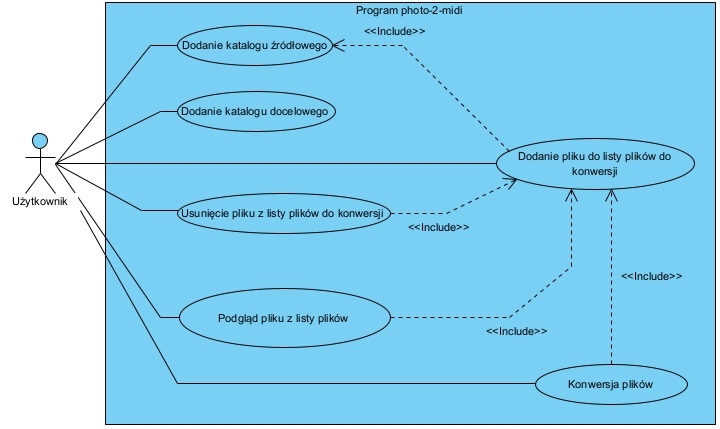
\includegraphics[width=14cm]{images/p2m-usecase-diagram}
	\caption{Diagram przypadków użycia}
	\label{fig:usecase-diagram}
\end{figure}

\noindent \textbf{Przypadek użycia:} Dodanie katalogu źródłowego\\
\textbf{Aktor:} Użytkownik\\
\textbf{Opis:} Wskazanie przez użytkownika katalogu zawierającego pliki przeznaczone do konwersji.\\
\textbf{Warunki wstępne:} -\\
\textbf{Przebieg:}
\begin{enumerate}
	\item Użytkownik klika przycisk "Browse" znajdujący się po lewej stronie.
	\item Otwiera się okno wyboru katalogu źródłowego.
	\item Użytkownik nawiguje do wybranego katalogu zawierającego pliki przeznaczone do konwersji.
	\item Użytkownik wybiera katalog zawierający pliki przeznaczone do konwersji.
	\item Użytkownik akceptuje wybrany katalog jako katalog źródłowy.
	\item Program wyświetla listę kompatybilnych plików z wybranego katalogu.
\end{enumerate}


\noindent \textbf{Przypadek użycia:} Dodanie katalogu docelowego\\
\textbf{Aktor:} Użytkownik\\
\textbf{Opis:} Wskazanie przez użytkownika katalogu docelowego.\\
\textbf{Warunki wstępne:} -\\
\textbf{Przebieg:}
\begin{enumerate}
	\item Użytkownik klika przycisk "Browse" znajdujący się po prawej stronie.
	\item Otwiera się okno wyboru katalogu docelowego.
	\item Użytkownik nawiguje do wybranego katalogu.
	\item Użytkownik wybiera katalog przeznaczony do zapisu wyników konwersji.
	\item Użytkownik akceptuje wybrany katalog jako katalog docelowy.
	\item Program dodaje wybrany katalog jako katalog docelowy.
\end{enumerate}


\noindent \textbf{Przypadek użycia:} Dodanie pliku do listy plików do konwersji\\
\textbf{Aktor:} Użytkownik\\
\textbf{Opis:} Dodanie pliku znajdującego się w wybranym katalogu źródłowym do listy plików przeznaczonych do konwersji.\\
\textbf{Warunki wstępne:} Katalog źródłowy został wybrany przez użytkownika i zawiera co najmniej jeden kompatybilny plik.\\
\textbf{Przebieg:}
\begin{enumerate}
\item Użytkownik zaznacza wybrany plik z listy plików znajdujących się w katalogu źródłowym.
\item Użytkownik używa przycisku oznaczonego znakiem \textbf{> >}, by przenieść wybrany plik do listy plików przeznaczonych do konwersji.
\item Program przenosi wybrany plik do listy plików przeznaczonych do konwersji.
\end{enumerate}


\noindent \textbf{Przypadek użycia:} Usunięcie pliku z listy plików do konwersji\\
\textbf{Aktor:} Użytkownik\\
\textbf{Opis:} Usuwanie pliku znajdującego się w liście plików przeznaczonych do konwersji.\\
\textbf{Warunki wstępne:} Co najmniej jeden plik znajduje się w liście plików do konwersji.\\
\textbf{Przebieg:}
\begin{enumerate}
	\item Użytkownik zaznacza wybrany plik z listy plików przeznaczonych do konwersji.
	\item Użytkownik używa przycisku oznaczonego znakiem \textbf{DEL}, by usunąć wybrany plik z listy plików przeznaczonych do konwersji.
	\item Program usuwa wybrany plik z listy plików przeznaczonych do konwersji.
\end{enumerate}


\noindent \textbf{Przypadek użycia:} Podgląd plików z listy plików\\
\textbf{Aktor:} Użytkownik\\
\textbf{Opis:} Wyświetlenie podglądu wybranego pliku z listy.\\
\textbf{Warunki wstępne:} Co najmniej jeden kompatybilny plik znajduje się w katalogu źródłowym lub co najmniej jeden plik został przeniesiony do listy plików przeznaczonych do konwersji.\\
\textbf{Przebieg:}
\begin{enumerate}
	\item Użytkownik zaznacza wybrany plik na liście plików przeznaczonych do konwersji lub liście plików w katalogu źródłowym.
	\item Program wyświetla podgląd wybranego pliku.
\end{enumerate}


\noindent \textbf{Przypadek użycia:} Konwersja plików\\
\textbf{Aktor:} Użytkownik\\
\textbf{Opis:} Rozpoczęcie procedury konwersji plików.\\
\textbf{Warunki wstępne:} Co najmniej jeden plik znajduje się w liście plików do konwersji.\\
\textbf{Przebieg:}
\begin{enumerate}
	\item Użytkownik używa przycisku "Convert".
	\item Program wyświetla informację o rozpoczęciu działania.
	\item Po zakończonej konwersji program wyświetla informację o katalogu zawierającym wynik konwersji.
\end{enumerate}





\section{Interfejs graficzny}

Interfejs został stworzony przy użyciu biblioteki \textit{PySimpleGUI}.

\begin{figure}[h]
	\centering
	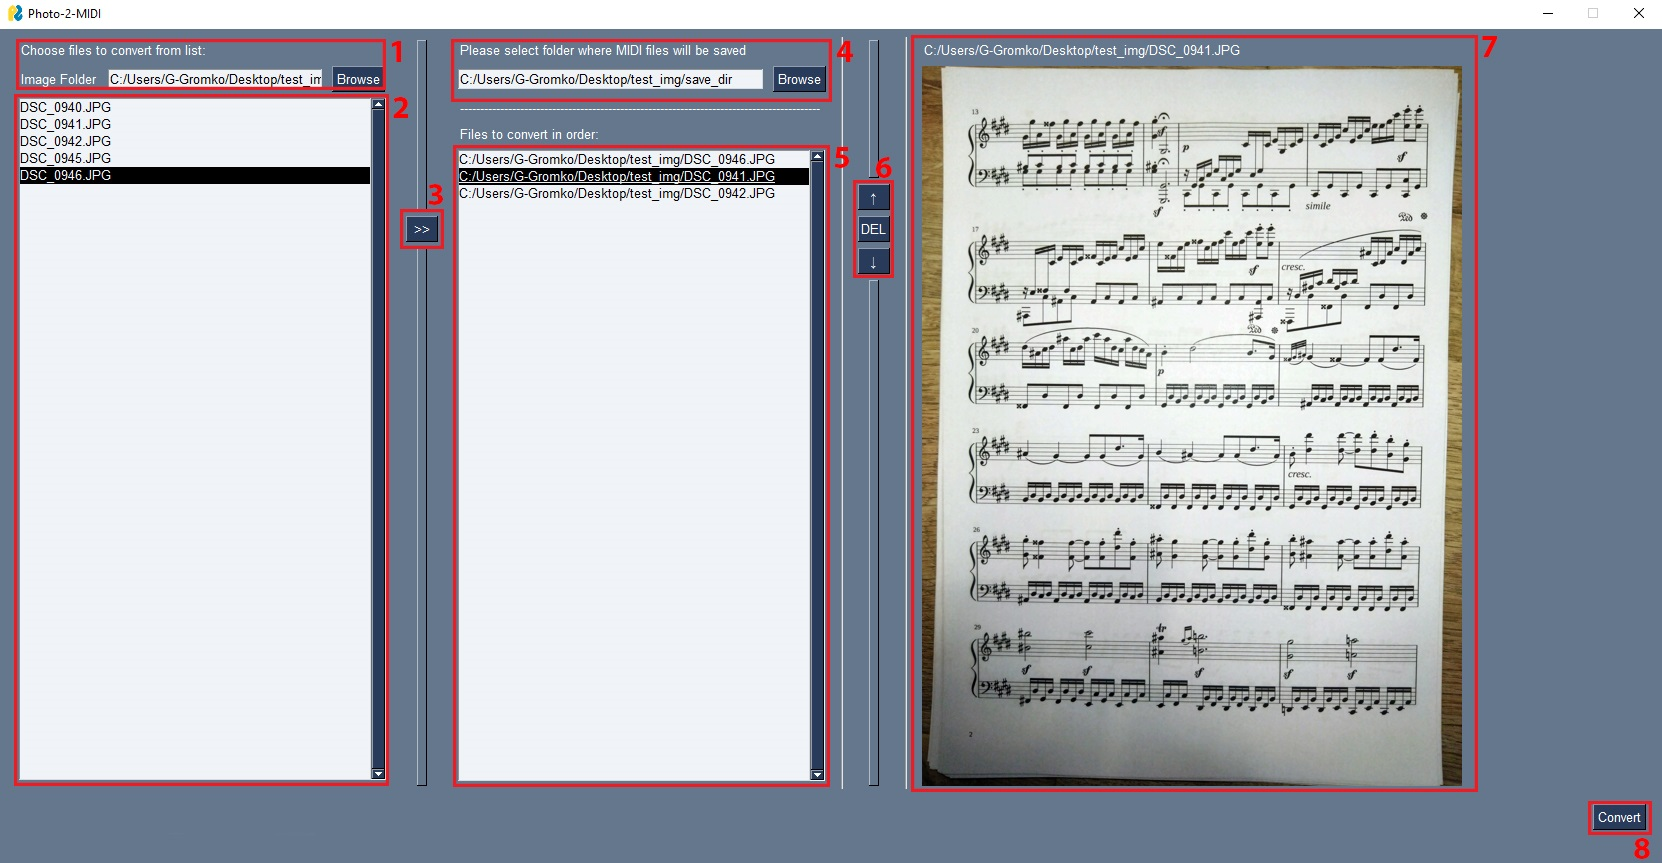
\includegraphics[width=16cm]{images/gui}
	\caption{Interfejs graficzny programu Photo-2-MIDI}
	\label{fig:gui}
\end{figure}

\begin{enumerate}
	\item Pole tekstowe do wprowadzenia ścieżki folderu ze zdjęciami zapisu nutowego.
	\item Lista plików w wybranym folderze.
	\item Przycisk do przeniesienia zaznaczonego pliku do listy plików do konwersji.
	\item Pole tekstowe do wprowadzenia ścieżki folderu do którego mają zostać zapisane uzyskane pliki MIDI.
	\item Lista plików przeznaczonym do konwersji, ułożone w kolejności w której konwersja ma się odbyć.
	\item Przyciski do organizacji plików przeznaczonych do konwersji, kolejno: przesuń wybrany plik w górę na liście, usuń wybrany plik z listy, przesuń wybrany plik w dół na liście.
	\item Podgląd wybranego pliku z jednej z list.
	\item Przycisk uruchamiający konwersję zdjęć do plików MIDI.
\end{enumerate}